\newpage

\subsection{Montaža stročnic}
Stroj deluje na principu kratko-stružnih stročnic. Zato vsebuje le eno stročnico,
katero je potrebno zamenjati. Ob menjavi je potrebnu tudi preveriti pritisk
stročnice, ki se nastavlja z matico. Če je pritisk prevelik, se stročnica veliko
hitreje obrabi in tudi pušča odtise na izdelku, če je pa premajhen pa obstaja možnost,
da podajalec potisne palico preko stročnice, ta se pa lahko zatakne med
premikajoče dele, uniči rezalne plošlice ali pa zlomi svedre.

Ko se ta nastavi je potrebno prilagoditi krivuljo, ki nadzira odpiranje in
zapiranje stročnice. Ta nam stročnico odpre, za tem se celoten zadnji suport
pomakne nazaj za dolžino kosa kjer se palica ponovno vpne. Medtem pa podajalec
čež celoten cikel potisne palico ob odrezni nož, da se ob premiku suporta ne premakne.

Potrebno je še izračunat čas, ki nam je na voljo za preprijem stročnice.
Ta se zračuna tako, da se od časa cikla odšteje ves skupni čas, potreben
za obdelavo po spodnji enačbi \ref{eq:13}:

\begin{equation}
	\label{eq:13}
	\begin{split}
		t_c &= t_{r1+r2} + t_{cent} + t_{vrt} + t_{odr} \\
		t_c &= 0.75s + 0.95s + 3.8s + 4.5s = 10s
	\end{split}
\end{equation}

Za vpetje in razpetje stročnice stroj potrebuje približno 0.2s, za premik
suporta, pa približno 0.5-0.8s. Ker je skupen čas za obdelavo kosa
enak času enega obrata krivuljne gredi, bo potrebno nekatere obdelave
nastaviti, da se prekrivajo med sabo. Npr. v našem primeru je možno
nastaviti, da se čas pobiranja robov in centriranja prekriva in
nam omogoča ravno dovolj časa za cikel vpetja.

Stroj GM127 uporablja stročnico z dimenzijami na sliki \ref{slika_strocnice},
katero je možno izdelati tudi na stružnici.

\begin{figure}[H]
	\begin{center}
		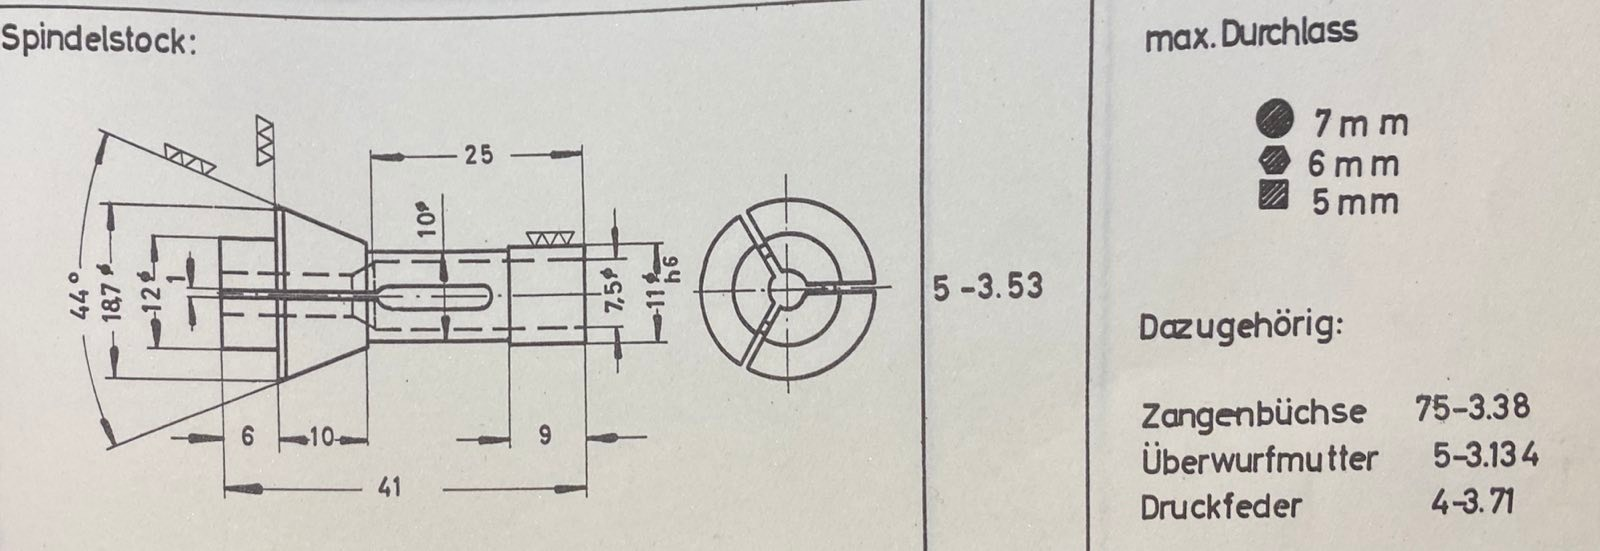
\includegraphics[width=\linewidth]{slika_strocnice.jpg}
		\caption{Slika dimenzij stročnice iz priročnika
			stroja Gauthier GM127 pod prilogo VI
			\cite{gauthier}}
		\label{slika_strocnice}
	\end{center}
\end{figure}

Stročnica vpne material zaradi sprednjega konusa, na katerega
pritisne posebna puša z nasprotno postruženim konusom. Sprednji
del stročnice je fiksiran z matico, ki preprečuje aksialni pomik,
kadar jo puša pritisne. Sistem je zelo zanimiv, saj imamo dve
puše znotraj cevi, ena je premična, ena pa fiksna. Fiksna puša
vodi material iz podajalca skozi celotno vreteno in ima tudi
ležišče, kamor se stročnica prilega. Premična puša pa preko
posebnih vpenjalnih prstov prenese silo iz krivulje na stročnico.